\chapter{Evaluierung}
\label{chap:eval}
\todo[size=\small, color=blue!40, inline]{Kapitel: Evaluierung}%
\begin{itemize}
 \item wie skaliert das System / bringt es was?
 \item Cache löschen - neu laden -> Zeit messen
 \item Verschiedene Kamerapositionen:
 \begin{itemize}
  \item Turbine
  \item Cockpit
  \item Heck
  \item ``Businessclass''
  \item seitlich von Außen
 \end{itemize}
 \item Erklärung der Tests \& Diagramme
 \item Balancierung durch c-Collision Protokoll / die Varianz
\end{itemize}
\todo[size=\small, inline]{Grafiken mit echten Daten füllen!}%




\begin{figure}
\centering
%%%%%%%%%%%%%%%%%%%%%%%%%%%%%%%%%%%%%%%%%%%%%%%%%%%%%%%%%
% Beispieldiagramm mit pgfplot und datenfile
%%%%%%%%%%%%%%%%%%%%%%%%%%%%%%%%%%%%%%%%%%%%%%%%%%%%%%%%%

\begin{tikzpicture}
  \begin{axis}[xlabel=$x$, ylabel={$f(x) = x^2 - x +4$}]
    \addplot table[col sep=comma,x index=0,y index=2,header=false] {data/data.dat};
    \addlegendentry{model}
    \addplot coordinates {
      (-4.77778,2027.60977)
      (-3.55556,347.84069)
      (-2.33333,22.58953)
      (-1.11111,-493.50066)
      (0.11111,46.66082)
      (1.33333,-205.56286)
      (2.55556,-341.40638)
      (3.77778,-1169.24780)
      (5.00000,-3269.56775)
    };
    \addlegendentry{dfsda}
  \end{axis}
\end{tikzpicture}

  \caption{Ein Beispieldiagramm mit Datenfile.}
  \label{fig:eval:diag1}
\end{figure}

\begin{figure}
\centering
\input{plots/diag2.tex}
  \caption{Beispieldiagramm 2.}
  \label{fig:eval:diag2}
\end{figure}

\begin{figure}
\centering
%%%%%%%%%%%%%%%%%%%%%%%%%%%%%%%%%%%%%%%%%%%%%%%%%%%%%%%%%
% Testdiagramm 3
%%%%%%%%%%%%%%%%%%%%%%%%%%%%%%%%%%%%%%%%%%%%%%%%%%%%%%%%%


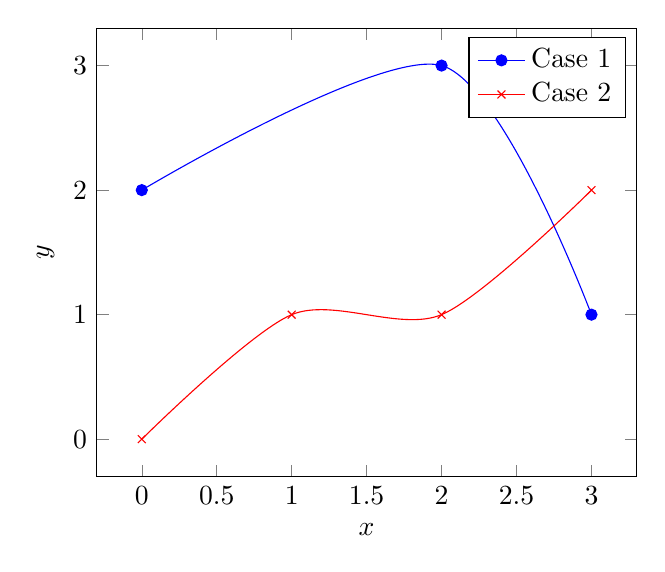
\begin{tikzpicture}
  \begin{axis}[xlabel=$x$, ylabel=$y$]
    \addplot[smooth,mark=*,blue] plot coordinates {
      (0,2)
      (2,3)
      (3,1)
    };
    \addlegendentry{Case 1}
    \addplot[smooth,color=red,mark=x]
        plot coordinates {
            (0,0)
            (1,1)
            (2,1)
            (3,2)
        };
    \addlegendentry{Case 2}
  \end{axis}
\end{tikzpicture}

  \caption{Beispieldiagramm 3.}
  \label{fig:eval:diag3}
\end{figure}

\begin{figure}
\centering
\input{plots/diag4.tex}
  \caption{Beispieldiagramm 4.}
  \label{fig:eval:diag4}
\end{figure}

